\section{Problem Formulation and Motivation}
This section first formulates the problem statement in Section~2.1. Section~2.2 then presents two key observations that motivate our design,
 namely temporal locality across updates and skew in practical query workloads. Finally, Section~2.3 discusses the main challenges in designing BriskSeed.

\subsection{Problem Statement}

We begin with the standard Approximate Nearest Neighbor Search(ANNS) definition and then extend it to the dynamic setting considered in this paper.

\begin{table}[thb]
  \caption{Summary of terminologies}
  \label{tab:symbols}
  \begin{tabular}{lp{6.3cm}}
    \toprule
    Symbol & Description\\
    \midrule
    $\mathcal{D}$ & Vector dataset. \\
    $\mathcal{D}_r$ & Vector dataset state after applying the batch updates at round $r$. \\
    $\widehat{N}_k(q)$ & Approximate top-$k$ result set of query $q$. \\
    $N_k^{\ast}(q)$ & Exact top-$k$ nearest-neighbor set of query $q$. \\
    $\mathrm{Recall@}k(q)$ & Recall of the approximate top-$k$ result for query $q$. \\
    $\mathcal{U}_r$ & Batch updates at round $r$. \\
    $\mathcal{Q}_r$ & Batch queries executed at round $r$. \\
	$\mathcal{R}$ & The number of rounds we evaluate. \\
    $L_{\mathrm{search}}(q)$ & Search latency of query $q$. \\
    $L_{\mathrm{maintain}}(\mathcal{U}_r)$ & Maintenance cost triggered by batch updates $\mathcal{U}_r$. \\
    $\mathrm{QPS}(R)$ & Average query throughput within $\mathrm{R}$ rounds. \\
    $\tau$ & Tolerance threshold for Recall@$k$. \\
    \bottomrule
  \end{tabular}
\end{table}

\noindent\textbf{Definition 1 (ANNS).}
Given a vector dataset $\mathcal{D}\subset\mathbb{R}^d$, a query $q\in\mathbb{R}^d$, and an integer $k$, ANNS returns an approximate top-$k$ set $\widehat{N}_k(q)$ that approximates the exact nearest-neighbor set $N_k^{\ast}(q)$ under a distance metric. The standard search quality metric is Recall@$k$:
\begin{equation}
\mathrm{Recall@}k(q)=\frac{|\widehat{N}_k(q)\cap N_k^{\ast}(q)|}{k}.
\end{equation}

Definition 1 captures the static ANNS setting, where the vector dataset and index structure remain fixed during queries. 
In practical systems, however, vectors are continuously inserted and deleted, and therefore the ANNS index also evolves over time. 
To model this setting, we extend ANNS to a dynamic formulation and adopt the serialized round-based execution model used in CANDOR-Bench.

\noindent\textbf{Definition 2 (Dynamic ANNS).}
Dynamic ANNS operates on a time-evolving dataset in rounds. At each round $r$, the system first applies a batch updates $\mathcal{U}_r$ (insertions/deletions) 
to transform $\mathcal{D}_{r-1}$ into $\mathcal{D}_r$, and then executes a batch queries $\mathcal{Q}_r$ on $\mathcal{D}_r$. The index structure is updated online across rounds.

In this setting, many optimizations developed for static ANNS become less effective as updates accumulate, including layout restructuring, quantization-based acceleration, 
and globally precomputed auxiliary guidance. As their effectiveness decays, query throughput drops and recall may also deteriorate. Frequent re-optimization is not a viable
solution either, because its maintenance overhead can dominate end-to-end cost, as shown in Figure~\ref{fig:reopt-cost}. This dilemma motivates the following problem.

\noindent\textbf{Problem Statement.}
The goal is to maximize end-to-end query throughput in dynamic ANNS under continuous updates, while preserving comparable recall to baselines. In dynamic ANNS, low query latency is meaningful 
only if the maintenance required to sustain it is also affordable. We therefore account for both search cost and maintenance cost in the end-to-end throughput objective across update-query rounds.

Let $\mathcal{Q}_r$ denote the query batch at round $r$, and let $n_r = |\mathcal{Q}_r|$ be the number of queries in that round. Over an evaluation horizon of $R$ rounds, we define the total search cost and total maintenance cost as
\begin{equation}
L_s(R)=\sum_{r=1}^{R}\sum_{q\in\mathcal{Q}_r} L_{\mathrm{search}}(q), \quad L_m(R)=\sum_{r=1}^{R} L_{\mathrm{maintain}}(\mathcal{U}_r).
\end{equation}
The corresponding query throughput is
\begin{equation}
\mathrm{QPS}(R)=\frac{\sum_{r=1}^{R} n_r}{L_s(R)+L_m(R)}.
\end{equation}

Our objective is to maximize $\mathrm{QPS}(R)$ subject to an average recall constraint:
\begin{equation}
\begin{aligned}
\max \quad & \mathrm{QPS}(R) \\
\text{s.t.}\quad &
\frac{1}{\sum_{r=1}^{R} n_r}
\sum_{r=1}^{R}\sum_{q\in\mathcal{Q}_r}\mathrm{Recall@}k(q)
\ge
\tau \cdot \overline{\mathrm{Recall}}^{\mathrm{baseline}},
\end{aligned}
\end{equation}
where
\begin{equation}
\overline{\mathrm{Recall}}^{\mathrm{baseline}}=
\frac{1}{\sum_{r=1}^{R} n_r}
\sum_{r=1}^{R}\sum_{q\in\mathcal{Q}_r}\mathrm{Recall@}k(q)^{\mathrm{baseline}},
\end{equation}
and $\tau \in (0,1]$ controls the required recall ratio relative to the baseline.


\begin{figure}
	\centering
	\subfloat[Overlapped top-$k$ results across updates]{
		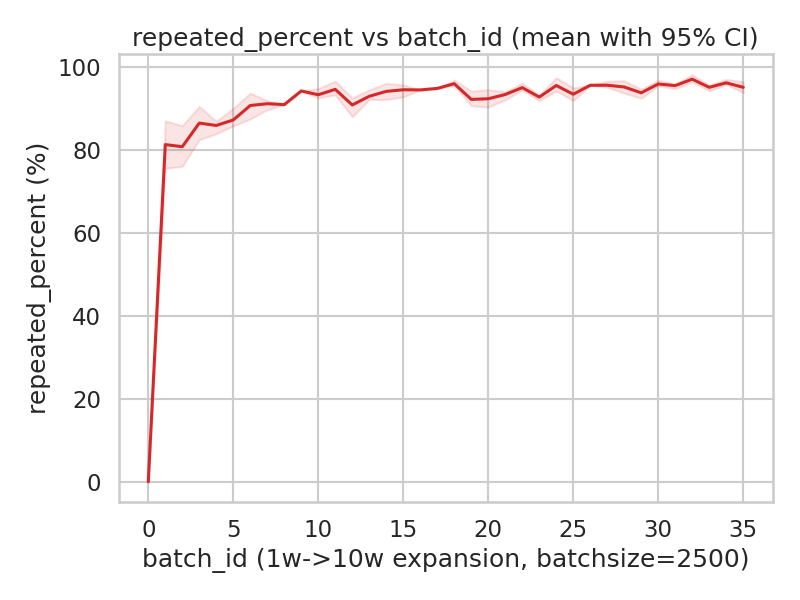
\includegraphics[width=0.48\columnwidth]{figures/figure2a.png}
		\label{fig:repeat results}
	}
    \subfloat[Skewness in query hotspot distribution]{
		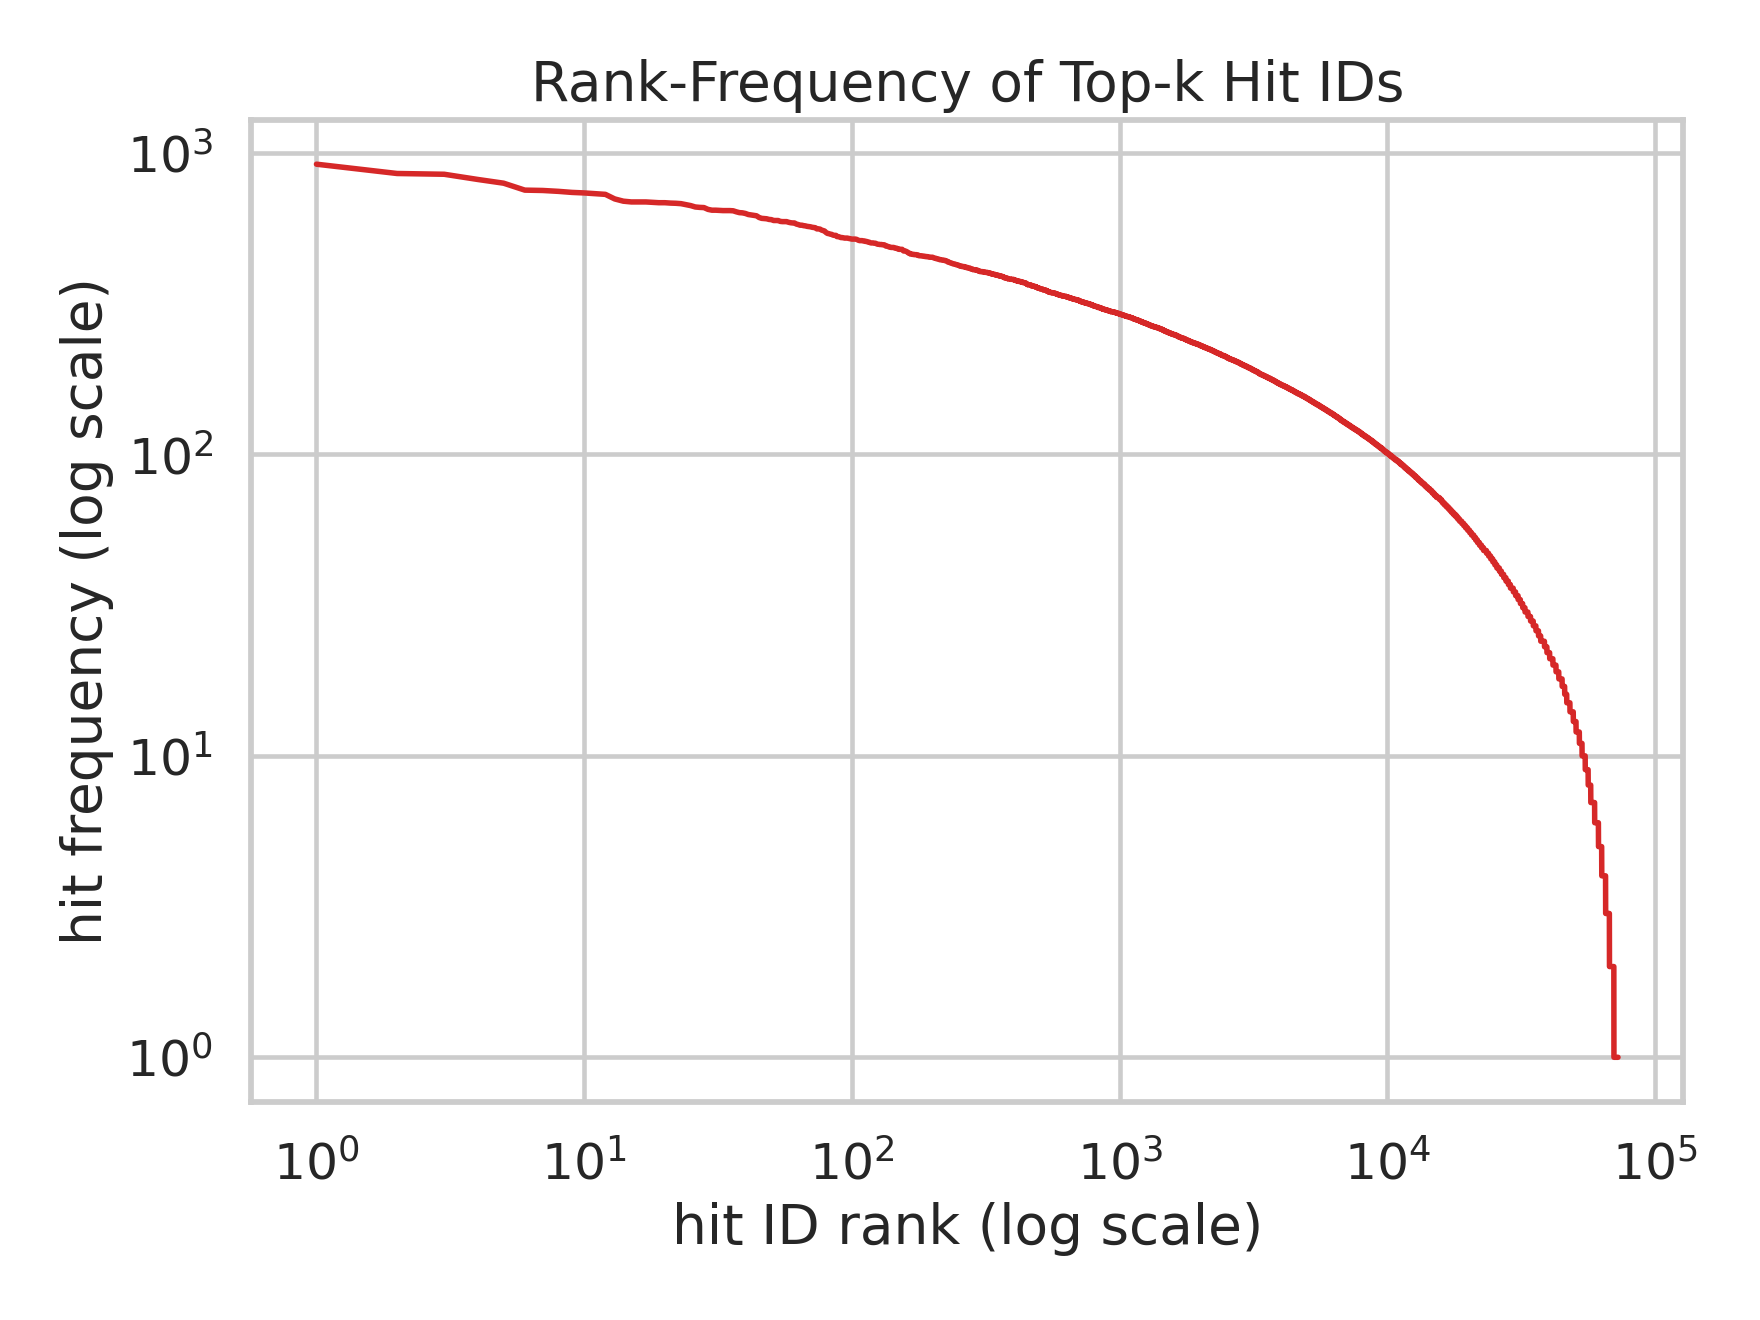
\includegraphics[width=0.48\columnwidth]{figures/figure2b.png}
		\label{fig:skewness}
	}
    \caption{Key observations in dynamic ANNS.}
	\label{fig:observation}
\end{figure}

\subsection{Key Observations}

To better understand the behavior of dynamic ANNS workloads, we conduct a preliminary empirical study and identify two key observations.

\noindent\textbf{Observation 1: Temporal locality across updates.} For the same query batch, the top-$k$ results often remain highly overlapping across nearby update rounds. 
As shown in Figure~\ref{fig:repeat results}, the 
overlap ratio of top-$k$ results quickly exceeds 80\% after the first few batches and remains around 95\% thereafter. This pattern indicates a form of 
\emph{temporal locality across updates}: although accumulated updates may gradually reduce the effectiveness of search acceleration, they do not immediately cause large 
changes in the query results. Therefore, recent high-quality search outcomes can potentially be reused for subsequent queries, as long as their 
reuse is bounded and adaptive.

\noindent\textbf{Observation 2: Long-tail skew in query-hit frequency.}
Across batch queries, the top-$k$ hit IDs often exhibit strong concentration rather than uniform coverage. As shown in Figure~\ref{fig:skewness}, the frequency 
of hit IDs follows a clear long-tail distribution: a small fraction of IDs is found very frequently, while the majority is rarely observed. This skew indicates 
that query-hit patterns in dynamic ANNS are highly uneven, and that not all recurring search outcomes are equally valuable for reuse. As a result, treating 
historical outcomes discriminately is likely to be cost-effective.


Taken together, these observations reveal both an opportunity and a principle for dynamic acceleration. Temporal locality suggests that recent search outcomes can be reused across updates, while long-tail skew suggests that such reuse should be selective rather than uniform. Therefore, an effective dynamic ANNS system should support both online reuse and cost-aware prioritization.


\subsection{Design Challenges}

Although the observations above reveal clear opportunities for dynamic ANNS acceleration, exploiting them efficiently and robustly under continuous updates remains non-trivial,
with the following challenges:

\noindent\textbf{Challenge 1: How should historical search outcomes be represented and stored?}
Although Observation 1 suggests that recent top-$k$ results can remain useful across nearby update rounds, high overlap does not imply that past outcomes can be reused unchanged. 
Instead, they should be retained as lightweight guidance for future search.
Therefore, the system must decide what information should be preserved from previous queries, how to represent it compactly, and how to store it under bounded memory overhead. 
Moreover, it must also balance retention and eviction so that useful outcomes remain available while stale ones are removed over time.

\noindent\textbf{Challenge 2: How can historical outcomes guide the search process?}
Even when historical outcomes are stored, turning them into effective search guidance remains non-trivial. 
The system must activate relevant outcomes for queries that do not exactly match previous ones, and use them to recover strong candidates without causing excessive search expansion. 
Moreover, Observation 2 suggests that reuse should be selective rather than uniform: highly recurring outcomes and long-tail outcomes may need to be handled differently in order to achieve good performance under bounded cost.
But, how to design such a selective reuse mechanism that can adapt to changing query-hit patterns is an open question.

\noindent\textbf{Challenge 3: How can historical-outcome reuse improve end-to-end query efficiency while preserving recall?}
Even when historical outcomes are well represented and selectively prioritized for search, reuse does not automatically improve both overall performance and recall, because the identified historical outcomes may still not reliable for current search. 
The system must therefore decide whether the reused search path should be accepted or whether it should fall back to the native search path, while keeping this decision process sufficiently lightweight. 
Designing such an acceptance-and-fallback mechanism is critical to ensuring that historical-outcome reuse improves efficiency without degrading recall.

Motivated by these challenges, we next present our design BriskSeed and elaborate on how it address Challenges 1-3.